% Chapter Template

\chapter{FDTD - One-Dimensional Scenario} % Main chapter title

\label{Chapter2} % Change X to a consecutive number; for referencing this chapter elsewhere, use \ref{ChapterX}

In this chapter, we will go more in depth into developing an application that can generate electromagnetic data in a one-dimensional domain. In the previous chapter, we mentioned a series of steps to implement FDTD, and that a part of them depend on the particular implementation. A keen eye will notice moving forward, that while the code will not change too much, each implementation deserves a different approach in the theoretical sense.

%----------------------------------------------------------------------------------------
%	SECTION 1
%----------------------------------------------------------------------------------------

\section{1D Discretization}

In the previous chapter, we ended up with the equations \ref{eqn:electricUpdateIntegral} and \ref{eqn:magneticUpdateIntegral}. They will now be used to do a FDTD discretization for the one-dimensional electromagnetic wave scenario. At the end of this section, we will have the update equations that we will use in our loops. Before moving on, we must first briefly discuss Transverse modes. A transverse mode is the type of pattern that an electromagnetic field, which is perpendicular with respect to the direction of the wave's propagation, has. For electromagnetic waves, the most relevant modes are TE (Transverse Electric) and TM (Transverse Magnetic). In our scenario, we will be using TEM mode for discretization, meaning neither electric nor the magnetic field are moving in the direction of propagation.

%-----------------------------------
%	SUBSECTION 1
%-----------------------------------
\subsection{Spatial and Temporal Shift}

The first step of the FDTD discretization is a shift in spacetime of the electric and magnetic fields. This spatial shift is shown in Figure \ref{fig:fdtd1dDiscretized}.

\begin{figure}
	\centering
	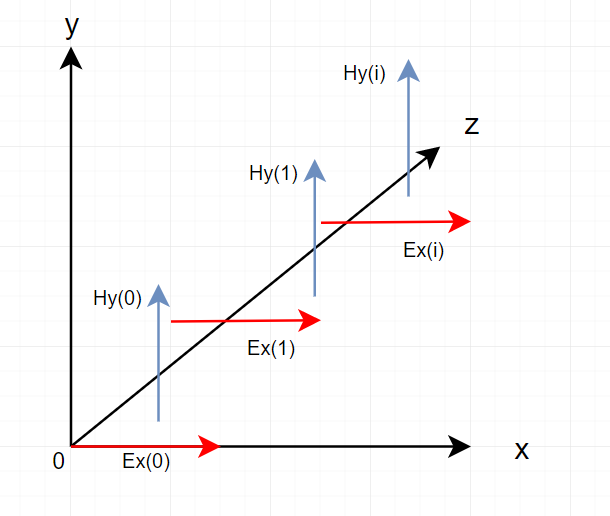
\includegraphics[scale=0.7]{Figures/fdtd1dDiscretized}
	\decoRule
	\caption[1D Spatial and Temporal Shift - TEM Mode]{The spatial and temporal shift of a one-dimensional electromagnetic scenario.}
	\label{fig:fdtd1dDiscretized}
\end{figure}

The electric vectors E are parallel to the x axis, while the magnetic vectors H are parallel to the y axis. The z axis in this case is the direction of the wave propagation.

%-----------------------------------
%	SUBSECTION 2
%-----------------------------------

\subsection{Electromagnetic Curls}

At first, the way that the vectors in Figure \ref{fig:fdtd1dDiscretized} are spaced out might seem odd. They look this way because they are part of each other's vector curl. We have two such curls in our one-dimensional scenario: one for the electric field vectors Ex,and one for the magnetic field vectors Hy. These curls are necessary for the update equations, because they explain the relationship between the electric fields and the magnetic ones.

\begin{figure}
	\centering
	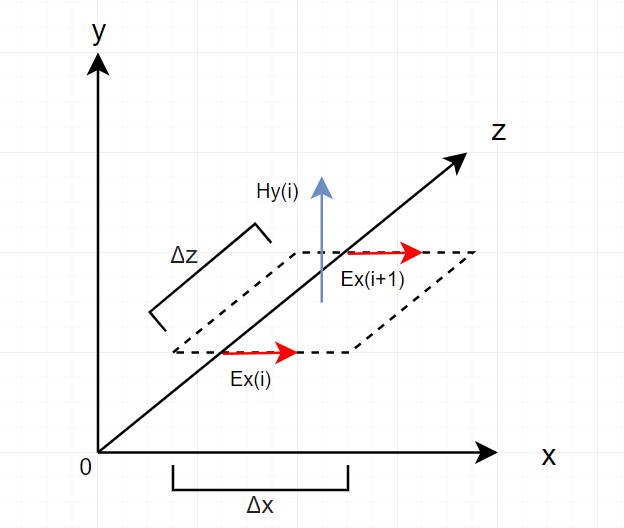
\includegraphics[scale=0.7]{Figures/fdtd1dHcurl}
	\decoRule
	\caption[1D Curl around $H_y$]{A graph showing the one-dimensional curl around the vector $H_y(i)$.}
	\label{fig:fdtd1dHcurl}
\end{figure}

Figure \ref{fig:fdtd1dHcurl} shows the curl around the magnetic vector $H_y(i)$. We can use this curl and plug it in to the original equation \ref{eqn:electricUpdateIntegral}:

\begin{equation}
	\label{eqn:magneticCurl1}
	\oint E \cdot ds = E_x(i) \cdot \Delta x + E_z \cdot \Delta z - E_x(i+1) \cdot \Delta x - E_z \cdot \Delta z
\end{equation}

Since we do not have an Ez vector in the one-dimensional scenario, $Ez \cdot \Delta z = 0$. Therefore we can simplify equation \ref{eqn:magneticCurl1} to:

\begin{equation}
	\label{eqn:magneticCurl2}
	\oint E \cdot ds = E_x(i) \cdot \Delta x - E_x(i+1) \cdot \Delta x
\end{equation}

On the left hand side of equation \ref{eqn:electricUpdateIntegral} we have:

\begin{equation}
	\label{eqn:magneticCurl3}
	\int \mu \cdot H \cdot dA = \mu \int H \cdot dA = \mu \cdot H_y(i) \cdot \Delta y \cdot \Delta z
\end{equation}

By combining \ref{eqn:magneticCurl2} and \ref{eqn:magneticCurl3}, we get:

\begin{equation}
	\label{eqn:magneticCurl4}
	\Delta x(E_x(i) - E_x(i+1)) = -\frac{d}{dt} (\mu \cdot H_y(i) \cdot \Delta y \cdot \Delta z)
\end{equation}

\begin{equation}
	\label{eqn:magneticCurl5}
	E_x(i) - E_x(i+1) = -\mu \cdot \Delta z \cdot \frac{dH_y(i)}{dt}
\end{equation}

We can do the same thing for the curl of the electric vector $E_x$, shown in Figure \ref{fig:fdtd1dEcurl}, as follows (Similar to the previous scenario, $H_z = 0$):

\begin{figure}
	\centering
	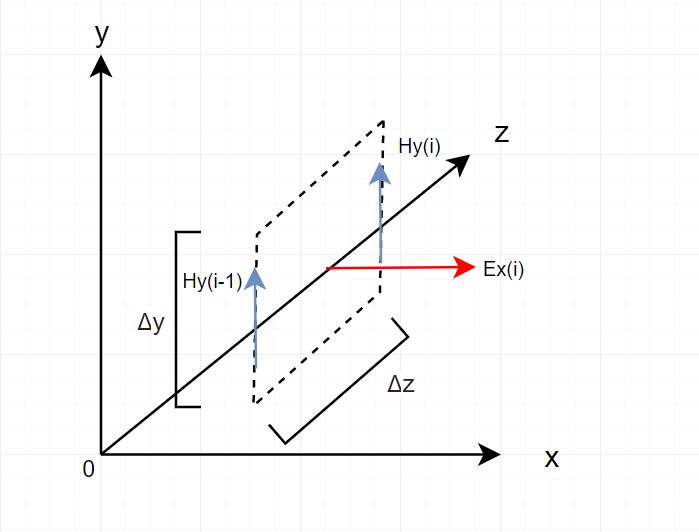
\includegraphics[scale=0.7]{Figures/fdtd1dEcurl}
	\decoRule
	\caption[1D Curl around $E_x$]{A graph showing the one-dimensional curl around the vector $E_x(i)$.}
	\label{fig:fdtd1dEcurl}
\end{figure}

\begin{equation}
	\label{eqn:electricCurl1}
	\oint H \cdot ds = H_y(i) \cdot \Delta y - H_y(i-1) \cdot \Delta y = \Delta y (H_y(i) - H_y(i-1))
\end{equation}

\begin{equation}
	\label{eqn:electricCurl2}
	\iint \epsilon \cdot E \cdot dA = \epsilon \cdot E_x(i) \cdot \Delta z \cdot \Delta y
\end{equation}

Combining \ref{eqn:electricCurl1} and \ref{eqn:electricCurl2}:

\begin{equation}
	\label{eqn:electricCurl3}
	\Delta y (H_y(i) - H_y(i-1)) = \frac{d}{dt} (\epsilon \cdot E_x(i) \cdot \Delta z \cdot \Delta y)
\end{equation}
\begin{equation}
	\label{eqn:electricCurl4}
	H_y(i) - H_y(i-1) = \epsilon  \cdot \Delta z  \cdot \frac{d}{dt} E_x(i)
\end{equation}

With those equations, we can now use the leapfrog time scheme to stagger our components along the time axis (Fig. \ref{fig:fdtd1dLeapfrog}).

\begin{figure}[!h]
	\centering
	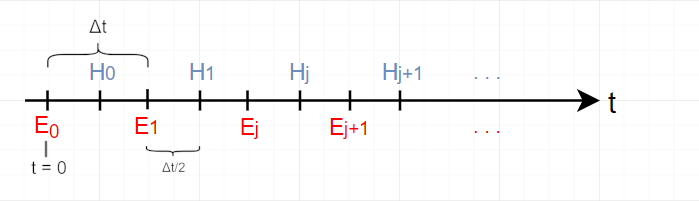
\includegraphics[scale=0.75]{Figures/fdtd1dLeapfrog}
	\decoRule
	\caption[Leapfrog Time Scheme]{Staggering the components along the time axis t using the leapfrog time scheme}
	\label{fig:fdtd1dLeapfrog}
\end{figure}

We will use the following indexing scheme:

\begin{equation}
	\label{eqn:indexingElectric}
	E_{i,j} = E(i \cdot \Delta z , j \cdot \Delta t)
\end{equation}

\begin{equation}
	\label{eqn:indexingMagnetic}
	H_{i,j} = H((i + \frac{1}{2}) \cdot \Delta z , (j + \frac{1}{2}) \cdot \Delta t)
\end{equation}

Using \ref{eqn:indexingElectric} and \ref{eqn:indexingMagnetic} we get the following time derivatives:

\begin{equation}
	\label{eqn:timeDerivativeE}
	\frac{d E_x}{dt} \bigg\rvert_{\underset{z = i \cdot \Delta z}{t=(j + \frac{1}{2})\Delta t}} = \frac{E_{x^{i,j+1}} - E_{x^{i,j}}}{\Delta t}
\end{equation}

\begin{equation}
	\label{eqn:timeDerivativeH}
	\frac{d H_y}{dt} \bigg\rvert_{\underset{z = (i + \frac{1}{2}) \Delta z}{t=j \cdot \Delta t}} = \frac{H_{y^{i,j}} - H_{y^{i,j-1}}}{\Delta t}
\end{equation}

Going back to equation \ref{eqn:magneticCurl5} we get:

\begin{equation}
	\label{eqn:timeDerivativeE2}
	E_x(i \cdot \Delta z) - E_x((i+1) \cdot \Delta z) = -\mu \cdot \Delta z \cdot \frac{d H_y((i+1/2)\Delta z) }{\Delta t}
\end{equation}

Evaluating at $t = j \cdot \Delta t$ gives us:

\begin{equation}
	\label{eqn:timeDerivativeE3}
	E_{x^{i,j}} - E_{x^{i+1,j}} = -\mu \cdot \Delta z \cdot \frac{H_{y^{i,j}} - H_{y^{i,j-1}}}{\Delta t}
\end{equation}

Finally, by solving for ${H_{y^{i,j}}}$ we get our update equation for the magnetic element:
	
\begin{equation}
	\label{eqn:magneticUpdate}
	H_{y^{i,j}} = H_{y^{i,j-1}} - \frac{\Delta t}{\mu \cdot \Delta z}(E_{x^{i,j}} - E_{x^{i+1,j}})
\end{equation}

In a similar way, we can get the update equation for the electric element by starting from the equation \ref{eqn:electricCurl4}. The result is:

\begin{equation}
	\label{eqn:electricUpdate}
	E_{x^{i,j+1}} = E_{x^{i,j}} + \frac{\Delta t}{\epsilon \cdot \Delta z}(H_{y^{i,j}} -  H_{y^{i-1,j}})
\end{equation}

Finally, we are ready to proceed into the code implementation.

%----------------------------------------------------------------------------------------
%	SECTION 2
%----------------------------------------------------------------------------------------

\section{C++ Implementation}

Calculating the update equations is by far the most difficult part of implementing FDTD. However, translating equations into code is not always straightforward. Before we begin the implementation, we need to prepare our coding environment. For this project, the author is using the Eclipse IDE for C++ Development\textsuperscript{\cite{eclipse}}. After creating a new project, we will start off with an empty skeleton that features the \textit{main()} method. Due to not needing any other classes, this is where we will place our code. Before that, we will need to include some packages so that we can use their methods, data types, and variables.

\begin{minted}[breaklines,frame=single,fontsize=\footnotesize]{c++}
#define _USE_MATH_DEFINES
	
#include <iostream>
#include <stdio.h>
#include <math.h>
#include <stdlib.h>
#include <cmath>
#include <vector>
#include <string>

using namespace std;
\end{minted}

To shortly explain what each line does:

\begin{itemize}
	\item \textbf{cmath, math.h}\textsuperscript{\cite{cmath}} - Packages that allow the use of various helpful math related commands and constants. Requires having \space \verb!#define _USE_MATH_DEFINES! set in order for everything to work properly
	\item \textbf{iostream, stdio.h}\textsuperscript{\cite{iostream}} - Allows for the usage of input and output stream objects and commands. In the 1D implementation, we will print our data to the console by using \verb!cout!
	\item \textbf{stdlib.h}\textsuperscript{\cite{cstdlib}} - Provides helpful data types, especially when dealing with vectors
	\item \textbf{vector}\textsuperscript{\cite{vector}} - Arrays in C++ are not dynamic. Once populated, they can no longer be modified. That is why for this implementation we need to use vectors.
	\item \textbf{string}\textsuperscript{\cite{string}} - Includes the string datatype. A string is basically an array of characters. Not only can we use this to format our output more easily, it can also be very useful for printing debugging messages.
\end{itemize}

Next, we will need to initialize some variables. To begin with, we need to set the permittivity $\epsilon$ and permeability $\mu$ of the domain that we are going to simulate. For our scenario, we are going to use $\epsilon_{0}$ and $\mu_{0}$, which are the values for vacuum.

\begin{minted}[breaklines,frame=single,fontsize=\footnotesize]{c++}
const double permitivity = 8.854e-12;  // vacuum permitivity
const double permeability = 1.256e-6;  // vacuum permeability
\end{minted}

These numbers are normally infinite, therefore we are already introducing inaccuracies into our simulation. For greater precision, we could include more decimals, though the difference would not be easily visible. Please note that although the units are not mentioned, we are using SI units for all calculations. This is important, as using the wrong unit could make the simulation inaccurate at best, or utterly unstable at worst.

\begin{minted}[breaklines,frame=single,fontsize=\footnotesize]{c++}
double L = 5;
int N = 200;
int iterNum = 800;
double deltaZ = L / N;
double deltaT = (deltaZ * sqrt(permitivity*permeability));
\end{minted}

\textbf{L} is the length of the domain in SI units, namely meters. \textbf{N} is the number of steps, or in the one-dimensional scenario the number of times we have sliced our domain. \textbf{iterNum} is the number of iterations. \textbf{deltaZ} ($\Delta z$) is the difference between the current step and the next one in meters. This can be set to anything, but we want to evenly split our domain and the best way to do so would be to set this to anything that is $x \cdot L/N$.

Special attention should be brought to \textbf{deltaT} ($\Delta t$). If this value is too big, the simulation will quickly grow unstable. While picking any arbitrary value would work, so long as it is small enough, we can choose a value that will always work through the equation below:

\begin{equation}
	\label{eqn:deltaTcode}
	\Delta t = \Delta z \cdot \sqrt{\epsilon \mu}
\end{equation}

This is the one-dimensional version of this equation. We will see how it changes later on when discussing the two-dimensional and three-dimensional scenarios. Now that our testing environment is ready, we will need to initialize the variables that will be used in our loops.

\begin{minted}[breaklines,frame=single,fontsize=\footnotesize]{c++}
// variables needed for Gaussian Pulse excitation
double eps = 1e-3;
double Teps = 50 * deltaT;
double beta = -(pow((2/Teps), 2) * log(eps));


vector<double> E;
vector<double> H;
vector<double> tE;
vector<double> tH;
\end{minted}

\textbf{E} and \textbf{H} are the electric and magnetic field vectors that will hold our data for each time step. For the one-dimensional scenario, in order to display the simulated data we will use what is called a time graph. A time graph is a graph of the values that an arbitrary point $n$ has during the simulation. We will choose the midpoint of the domain $N/2$ for our scenario, and the vectors \textbf{tE} and \textbf{tH} will contain the data of the electric and magnetic time graph respectively. We also initialize some helpful values that will be used by the Gaussian pulse excitation, with the equation \ref{eqn:gaussianPulse} mentioned in chapter \ref{Chapter1}: \textbf{eps} ($\varepsilon$), \textbf{Teps} ($T_\varepsilon$), and \textbf{beta} ($\beta$), with equation \ref{eqn:gaussianBeta} that was discussed in the same chapter.

We are done setting up the variables we will need for the simulation, therefore it is time to actually move on to the \textit{main()} method where we will implement the FDTD algorithm. First, we will need to populate our magnetic and electric field vectors, since we have not done so yet. Since we want our simulation to have no initial charge in it, we will have to set everything to $0$. Luckily there is a quick way to do so:

\begin{minted}[breaklines,frame=single,fontsize=\footnotesize]{c++}
E.assign(N, 0);
H.assign(N, 0);
\end{minted}

This will push N zeros to our vectors. Now we will need to start looping for \mint{c++}{int i = 0; i < iterNum; i++} values. We will also start off our Gaussian pulse here, by applying it to the beginning of the electric vector like so:

\begin{minted}[breaklines,frame=single,fontsize=\footnotesize]{c++}
double t = i * deltaT;
double gamma = Teps / 2;

E[0] = exp(-(beta * pow((t - gamma), 2)));
\end{minted}

Afterwards, we use the update equations that we derived above to get the values for the magnetic and electric fields:

\begin{minted}[breaklines,frame=single,fontsize=\footnotesize]{c++}
// loop for values
for (int z = 0; z < N-2; z++) {
	H[z] = H[z] - (deltaT / permeability / deltaZ) * (E[z] - E[z+1]);
}

for (int z = 1; z < N-1; z++) {
	E[z] = E[z] + (deltaT / permitivity / deltaZ) * (H[z] - H[z-1]);
}
\end{minted}

Please note that the starting index of a vector is zero, therefore when adding N values to our vectors, the index of the last value is going to be $N-1$. In our loops, we need to be certain that we never surpass this number. For the magnetic vector H loop, we need to make sure that the loop stops when $z + 1 = N - 1 \Leftrightarrow z = N - 2$. Alternatively, we could also populate $N + 1$ values, and extend our domain one unit past our boundaries.

After the above update loops, but while still inside the main loop, we will store the middle values into the respective time graph vectors for each time step:

\begin{minted}[breaklines,frame=single,fontsize=\footnotesize]{c++}
// time graph
tE.push_back(E[100]);
tH.push_back(H[100]);
\end{minted}

As mentioned previously, we can pick any point for this and it would still work. This is also another reasons why vectors are incredibly useful: we did not populate \textbf{tE} or \textbf{tH} with any values previously, therefore they had a length of zero. However, using the \textit{push\_back()} method, we can dynamically add values dynamically, therefore allowing us to change the number of iterations at will. 

After running the main loop \textbf{iterNum} times, we finally print our values to the console as a comma separated list:

\begin{minted}[breaklines,frame=single,fontsize=\footnotesize]{c++}
cout << "\n\ntE\n";

// print E values
for (int n = 0; n < iterNum; n++) {
	cout << to_string(tE[n]) + ",";
}

cout << "\n\ntH\n";

// print H values
for (int n = 0; n < iterNum; n++) {
	cout << to_string(tH[n]) + ",";
}
\end{minted}

The result is shown in figure \ref{fig:fdtd1dconsole}.

\begin{figure}[h!]
	\centering
	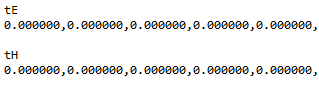
\includegraphics{Figures/fdtd1dconsole}
	\decoRule
	\caption[1D Console Output]{The console output of our FDTD one-dimensional algorithm}
	\label{fig:fdtd1dconsole}
\end{figure}

Now that we generated the data, we can proceed by choosing how to visualize it.

\section{Data Visualization}

Generating the data is the difficult part. In order to visualize it into a form that is easily understandable by humans, we can use a variety of programs. An easy solution for this is Microsoft Office Excel\textsuperscript{\cite{excel}}. While this software requires a license, there are viable alternatives to it that should be able to achieve the same results.

For starters, we will need to copy the comma separated list that is in our console output to the first column, in the second row for the electric data and the third row for the magnetic data. This will populate the first cell for both rows. After that, we can go to \textbf{Data > Text to Columns} and then split our one cell list into multiple columns (\ref{fig:fdtd1dexcel1}).

\begin{figure}[h!]
	\centering
	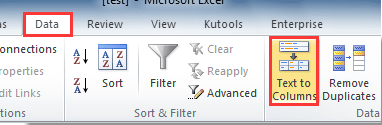
\includegraphics{Figures/fdtd1dexcel1}
	\decoRule
	\caption[1D Excel - Text to Columns]{Transforming data from a single cell containing the whole list, into separate columns for each value.}
	\label{fig:fdtd1dexcel1}
\end{figure}

After doing that for both electric and magnetic values, we can add a row of numbers above them for the timesteps. The result will look like so:

\begin{figure}[h!]
	\centering
	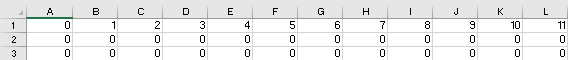
\includegraphics{Figures/fdtd1dexcel2}
	\decoRule
	\caption[1D Excel - Text to Columns]{Transforming data from a single cell containing the whole list, into separate columns for each value.}
	\label{fig:fdtd1dexcel2}
\end{figure}

With this, we can visualize the data however we desire. For the purposes of this demostration, we shall use line graphs. In Figure \ref{fig:emTimeGraph}, we have colored the time graph of the electric field orange, and the magnetic field blue.

\begin{figure}[h!]
	\centering
	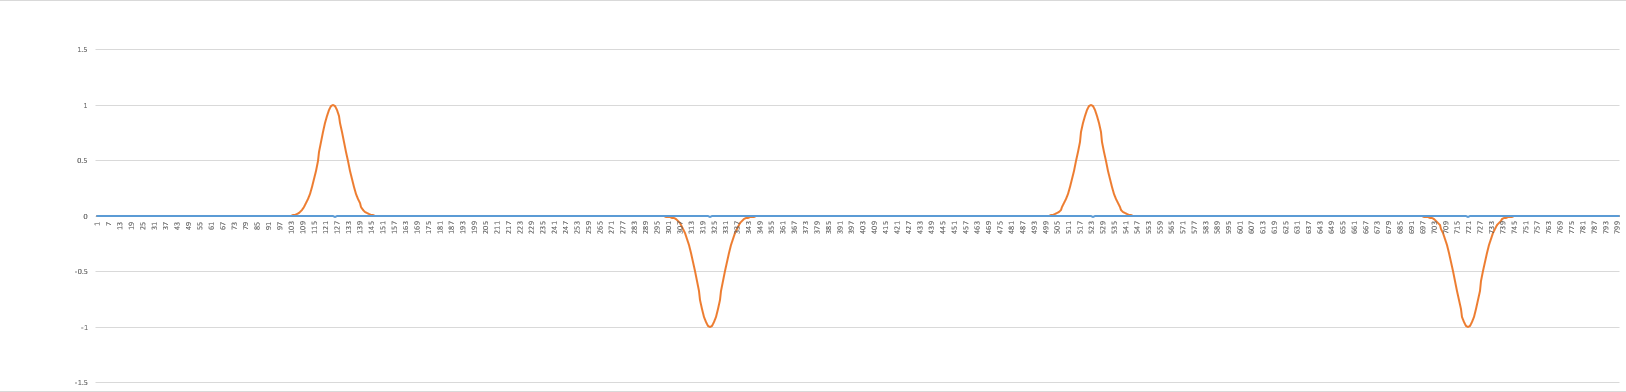
\includegraphics[scale=0.33]{Figures/1DtimeGraph}
	\decoRule
	\caption[1D Electromagnetic Time Graph]{The time graph of the electromagnetic data generated by our 1D application.}
	\label{fig:emTimeGraph}
\end{figure}

Please note that both lines were shown in the same plane due to convenience. The waves themselves move as they did during the discretization we did prior: electric waves move in the \textbf{X-Z} plane while the magnetic waves move in the \textbf{Y-Z} plane. Also, we can note that there is an enormous difference in the values of the electric and magnetic fields. We can easily tell that the electric wave is moving, but it is difficult to notice the magnetic wave movement. Here is one of those values zoomed in (Fig. \ref{fig:mTimeSnippet}):

\begin{figure}[h!]
	\centering
	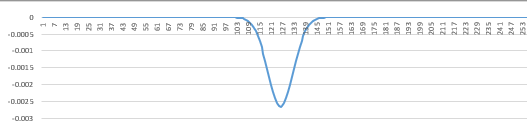
\includegraphics{Figures/1DmagneticTimeSnippet}
	\decoRule
	\caption[1D Magnetic Time Snippet]{A snippet of the time graph shown in Figure \ref{fig:emTimeGraph} zoomed in}
	\label{fig:mTimeSnippet}
\end{figure}

The reason for this difference being so big is due to the medium we chose for our domain: free space or otherwise known as vacuum. Also known as the impedance of free space, this value is commonly known as $Z_0 = $ \SI{376.730313668(57)}{\ohm}. This is also the ratio between the electric field and the magnetic one in free space. The value can also be calculated by using the permittivity and permeability:

\begin{equation}
	\label{eqn:impedance}
	Z_0 = \frac{E}{H} = \sqrt{\frac{\mu_0}{\epsilon_{0}}}
\end{equation}

With that done, let us take a look at the two-dimensional scenario.
	